\chapter{Minimax}\label{cap:minimax}

Minimax é um algoritmo que visa minimizar a perda máxima, isto é, dentre
o pior caso de cada possível decisão aquele que levar ao menor prejuízo.
Originalmente formulado para um jogo de soma zero de dois jogadores, o Minimax
já foi estendido para jogos mais complexos e decisões gerais em situações de
incerteza.

O princípio do minimax se aplica a um jogo $\Gamma=\langle A,B,H\rangle$ se a
equação~\ref{eq:req} for satisfeita, isto é, se existe uma valoração $v$ para o
jogo e uma estratégia ótima para ambos jogadores.
\cite{hazewinkel2002encyclopaedia}

\begin{gather}
  v=\max_{a\in A}\min_{b\in B}H(a,b)=\min_{b\in B}\max_{a\in A}H(a,b)\label{eq:req}
\end{gather}

Em que $A$ e $B$ são as estratégias dos jogadores 1 e 2 respectivamente e $H$ é a
função de utilidade que é positiva quando o jogador 1 está ganhando.

% TODO: explicar funcionamento
% TODO: Mostrar pseudo código

O algoritmo~\ref{lst:minimax} é um exemplo de pseudocódigo para o Minimax.

\begin{algorithm}
  \SetKwBlock{Procedimento}{Procedimento}{fim}
  \SetKwFunction{Utilidade}{Utilidade}
  \SetKwFunction{Proximos}{Próximos}
  \SetKwFunction{Valor}{Valor}

  \Entrada{$estado$, $jogador \in \{MIN, MAX\}$}
  \Saida{$decisão \in$ possíveis próximos estados}

  \Valor{$estado, jogador$} := \Inicio{%
    \Se{$estado$ é final}{%
      \Retorna{\Utilidade{$estado$}}\;
    }

    \eSe{$jogador$ = MAX}{%
      $valor \leftarrow$ máximo de $\Valor{proxEstado, MIN}: proxEstado \in \Proximos(estado)$\;
    }{% senão
      $valor \leftarrow$ mínimo de $\Valor{proxEstado, MAX}: proxEstado \in \Proximos(estado)$\;
    }
    \Retorna{$valor$}\;
  }

  \eSe{$jogador$ = MAX}{%
    $decisão \leftarrow proxEstado$ com máximo \Valor{$proxEstado, MIN$}\;
  }{% senão
    $decisão \leftarrow proxEstado$ com mínimo \Valor{$proxEstado, MAX$}\;
  }
  \Retorna{$decisão$}\;

  \caption{Pseudocódigo para tomada de decisão com o Minimax.}\label{lst:minimax}
\end{algorithm}

\section{Exemplo}

%A figura~\ref{fig:minimax-tree} exemplifica uma árvore de decisão usando esse
%método.
%
%\begin{figure}[ht]
%  \centering
%  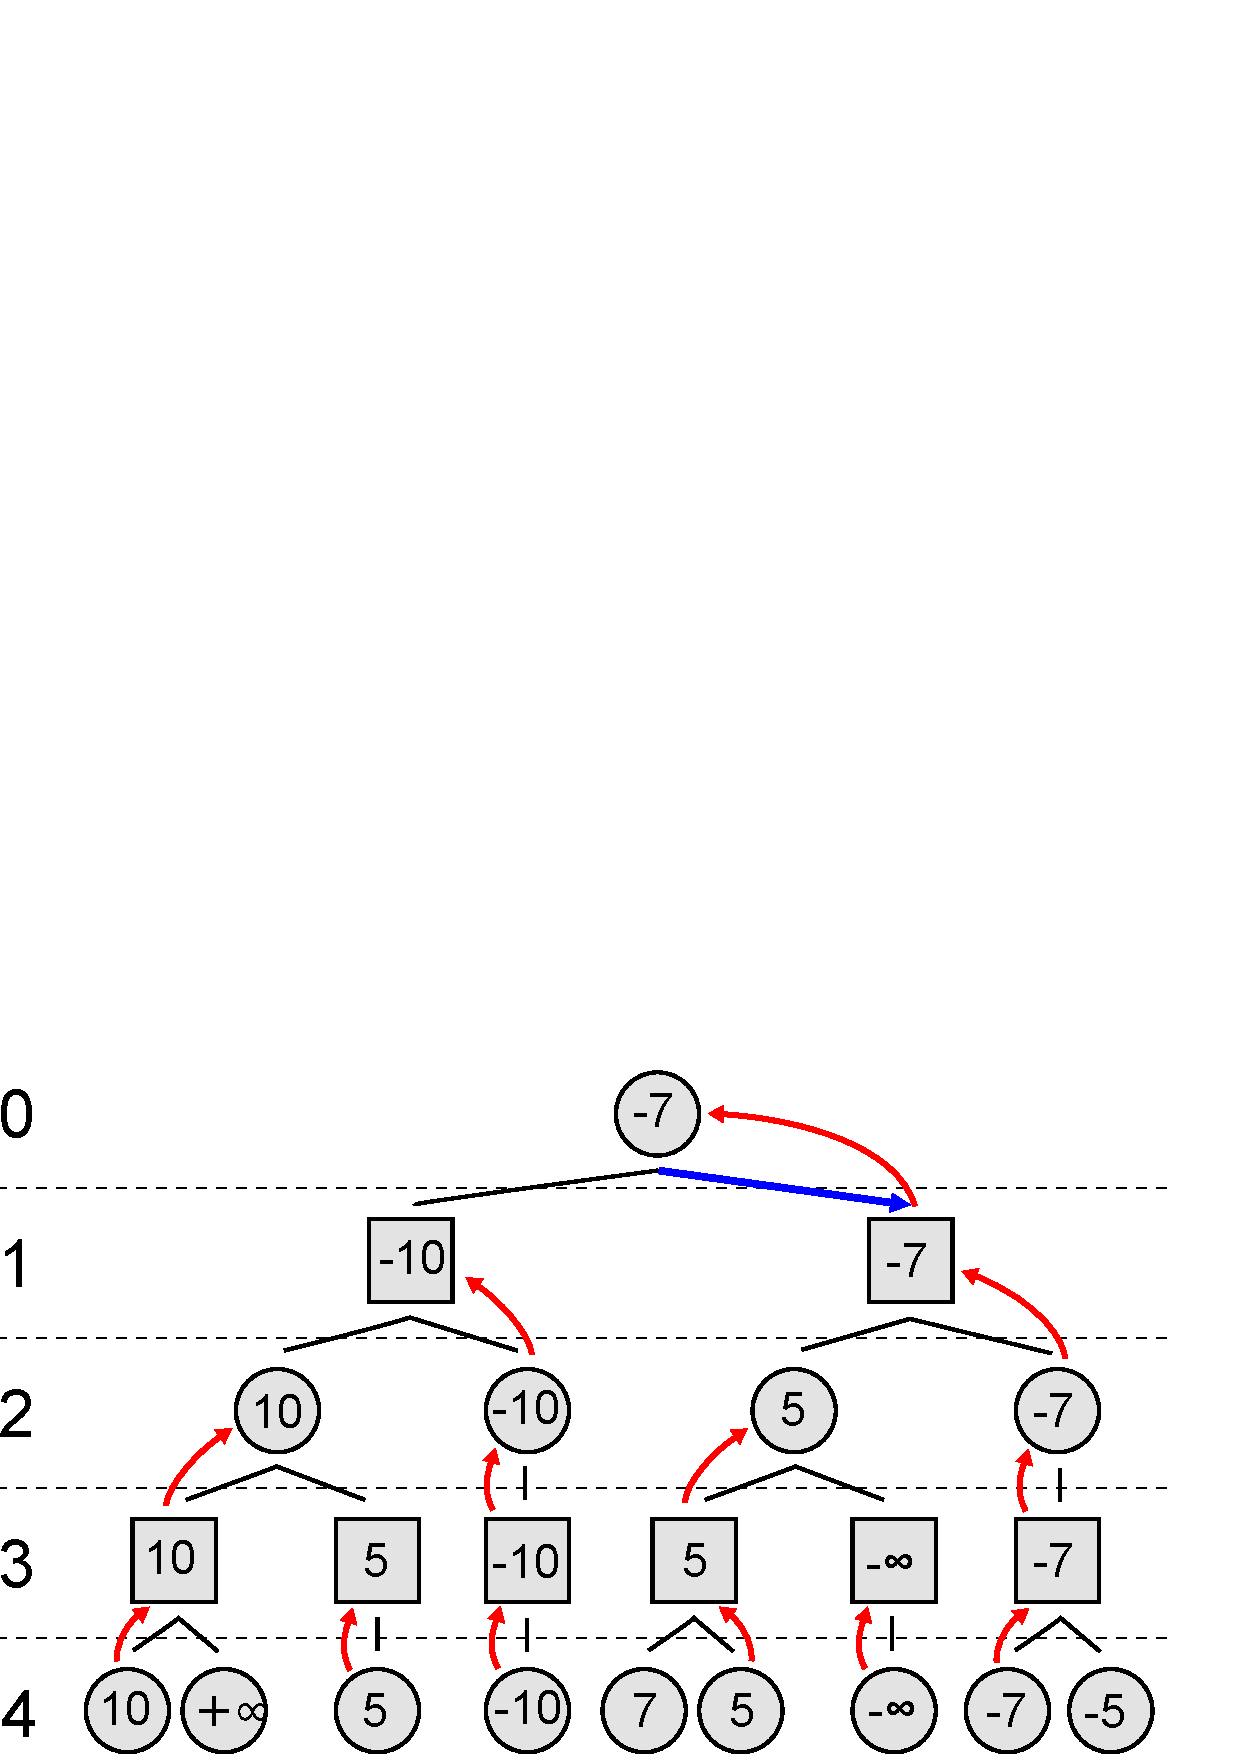
\includegraphics[width=0.7\linewidth]{minimax-tree}
%  \caption{Exemplo de árvore de decisão com Minimax.}\label{fig:minimax-tree}
%\end{figure}

O conhecido jogo da velha, que pode ser usado para exemplificar o algoritmo,
está representado na figura~\ref{fig:minimax-tictactoe}. Em que um valor $+1$
sinaliza uma vitória para o jogador $X$, $-1$ para o jogador $O$ e $0$, um
empate (ou velha).  Isto é o jogador $X$ é o $MAX$ e portanto $O$ o $MIN$.

Após aberta a árvore de jogadas e cada folha avaliada, nesse caso a avaliação
não é heurística pois o jogo é simples o suficiente para que isso não seja
necessário. A partir das folhas cada nó têm seu valor como o máximo dos valores
dos filhos quando é um nó $MAX$, e o mínimo quando $MIN$.

Assim a jogada imediata decidida pelo Minimax é a que tem valor $0$. Em termos
simplificados significa a jogada que na pior das hipóteses irá terminar em
velha.

\begin{figure}
  \centering
  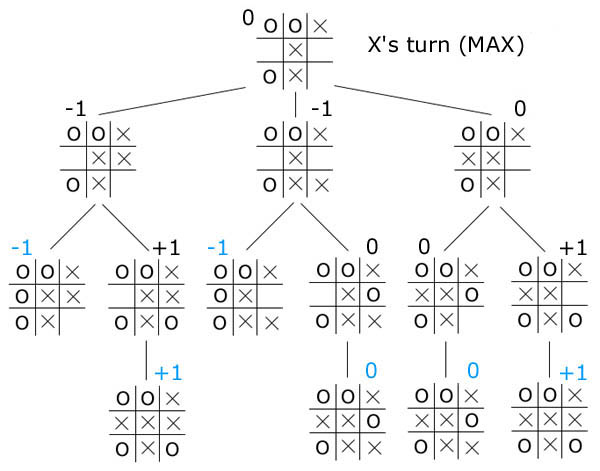
\includegraphics[width=0.7\linewidth]{minimax-tictactoe}
  \caption{Árvore do Minimax para o jogo da velha.}\label{fig:minimax-tictactoe}
\end{figure}

% vim: tw=80 et ts=2 sw=2 sts=2
